\documentclass[11pt]{article}
\usepackage[margin=1in]{geometry}
\usepackage{amsmath,amssymb}
\usepackage{booktabs}
\usepackage{graphicx}
\usepackage{multirow}
\usepackage{xcolor}
\usepackage{pgfplots}
\pgfplotsset{compat=1.17}
\usepackage{hyperref}
\usepackage[capitalise]{cleveref}
\usepackage{subcaption}
\usepackage{enumitem}

\definecolor{structblue}{RGB}{31,119,180}
\definecolor{logprobred}{RGB}{214,39,40}
\definecolor{surfacegray}{RGB}{127,127,127}
\definecolor{oraclegreen}{RGB}{44,160,44}

\title{Structural Self-Consistency for Quality Estimation\\in LLM-Based Information Extraction}

\author{Anonymous}
\date{}

\begin{document}
\maketitle

% ============================================================
% ABSTRACT
% ============================================================
\begin{abstract}
Large language models increasingly tackle structured information extraction (IE) via multi-sample generation, yet practitioners lack principled guidance on which confidence signals to trust---and for what purpose.
We systematically compare five unsupervised confidence signals spanning four families---model confidence (log-probability), surface agreement (Fleiss' $\kappa$, exact match), set-aware structural similarity (Soft Jaccard), and entity-level majority voting---for named entity recognition (NER) and relation extraction (RE) across two models (Qwen3-8B, LLaMA-3.1-8B) and two datasets (SciERC, CoNLL-2003).
We report three findings.
\textbf{(1)}~Structural consistency signals provide the strongest unsupervised quality estimation: entity voting achieves AUROC 0.73 and $\rho{=}0.50$ on NER, substantially outperforming log-probability (AUROC 0.56, $\rho{=}0.14$).
\textbf{(2)}~A \emph{correlation--selection gap} exists: despite strong instance-level correlation, no unsupervised signal beats greedy decoding for NER best-of-$N$ selection; only log-probability enables selection on RE (+2.4pp).
\textbf{(3)}~All signals degrade on relational tasks due to compound error propagation, but remain valid within the model's capability range.
These results hold across a $2{\times}2$ model--dataset matrix ($|\Delta\rho|{\le}0.006$ cross-model) and three random seeds ($\sigma_\rho{\le}0.008$).
Our findings disentangle quality estimation from sample selection and provide actionable guidance for deploying multi-sample IE systems.
\end{abstract}

% ============================================================
% 1. INTRODUCTION
% ============================================================
\section{Introduction}

Multi-sample generation---drawing $N$ candidate outputs from a language model and selecting or aggregating among them---has become a standard tool for improving LLM performance on reasoning tasks~\cite{wang2023selfconsistency,snell2024scaling,brown2024tts}.
For structured information extraction (IE), where outputs are entity sets or relation tuples, the natural question is: \emph{which confidence signal should guide the selection or abstention decision?}

This question is more nuanced than it appears.
Prior work on self-consistency~\cite{wang2023selfconsistency} uses exact-match voting, which conflates two distinct capabilities: (i)~\emph{quality estimation}---predicting which inputs yield reliable outputs---and (ii)~\emph{sample selection}---choosing the best output among $N$ candidates.
For structured outputs, surface-level agreement metrics further suffer from semantic blindness: two entity sets may differ in surface form yet agree structurally~\cite{nedellec2026consistency}.

We address these gaps with a systematic comparison of five confidence signals across four families for entity-level IE (\cref{sec:method}).
Our study spans two tasks (NER, RE), two models (Qwen3-8B, LLaMA-3.1-8B), two datasets (SciERC, CoNLL-2003), and evaluates both quality estimation (Spearman $\rho$, Kendall $\tau$, AUROC) and best-of-$N$ selection.

Our contributions are:
\begin{enumerate}[nosep,leftmargin=*]
\item We show that structural consistency signals---entity voting confidence and Soft Jaccard---are the strongest unsupervised quality estimators for IE, outperforming log-probability by 17--30 AUROC points and $0.2$--$0.4$ in Spearman $\rho$ (\cref{sec:results-qe}).
\item We identify a \emph{correlation--selection gap}: strong instance-level quality prediction does not translate to effective per-sample selection. On NER, no signal surpasses greedy decoding despite 16pp of oracle headroom (\cref{sec:results-gap}).
\item We characterize a \emph{task-complexity boundary}: compound error propagation in relational tasks degrades all consistency signals on the full instance set, but conditional filtering on the model's capability range restores discriminative power (\cref{sec:results-boundary}).
\item We validate these findings across a $2{\times}2$ model--dataset matrix with cross-model $|\Delta\rho|{\le}0.006$ and three-seed $\sigma_\rho{\le}0.008$ (\cref{sec:results-generalization}).
\end{enumerate}

% ============================================================
% 2. RELATED WORK
% ============================================================
\section{Related Work}

\paragraph{Self-consistency for reasoning.}
Wang et al.~\cite{wang2023selfconsistency} introduced self-consistency as majority voting over chain-of-thought samples, demonstrating gains on arithmetic and commonsense reasoning.
Subsequent work has extended this to confidence-weighted voting (CISC;~\citealt{cisc2025}), reliability-aware adaptive thresholds (ReASC;~\citealt{reasc2026}), sub-claim decomposition (Atomic Self-Consistency;~\citealt{atomic2024}), ranked voting~\cite{rankedvoting2025}, and KL-divergence-based reward-free selection~\cite{selfcertainty2026}.
All of these target discrete-answer reasoning tasks; none addresses the set-structured outputs characteristic of IE.

\paragraph{Uncertainty quantification for LLMs.}
Kuhn et al.~\cite{kuhn2023semantic} proposed semantic entropy over meaning-equivalent clusters.
Surveys by~\citet{uqsurvey2025} and~\citet{uqcalibsurvey2025} provide comprehensive taxonomies.
Semantic entropy probes~\cite{semanticprobes2024} and latent self-consistency~\cite{latentsc2025} reduce computational cost via embedding-space approximations.
Manakul et al.~\cite{manakul2023selfcheckgpt} use sampling-based self-checking for hallucination detection.
CoCoA~\cite{cocoa2025} combines confidence and consistency via minimum Bayes risk; Vashurin et al.~\cite{vashurin2025eval} systematically evaluate four UQ methods across tasks---none including structured IE.
Our work fills this gap by comparing confidence signal families specifically for entity-level and relational IE.

\paragraph{Calibration and selective prediction.}
Model calibration has been studied extensively~\cite{guo2017calibration,kadavath2022language,desai2020calibration}.
Selective prediction---abstaining on uncertain inputs---is surveyed by~\citet{geifman2017selective} and~\citet{knowyourlimits2025}.
The confidence estimation survey of~\citet{confestsurvey2024} provides a broad taxonomy.
For structured prediction, Kuleshov \& Liang~\cite{kuleshov2015structured} and Jagannatha \& Yu~\cite{jagannatha2022calibration} address calibration but not multi-sample consistency.
Our quality estimation results (\cref{sec:results-qe}) directly apply to selective prediction / abstention.

\paragraph{Confidence in information extraction.}
Culotta \& McCallum~\cite{culotta2004confidence} studied confidence estimation for CRF-based IE.
For NER, token-level uncertainty methods include MC-dropout~\cite{gal2016dropout,xiao2019quantifying} and deep ensembles~\cite{lakshminarayanan2017simple,shelmanov2021certain}.
N\'{e}dellec \& Xia~\cite{nedellec2026consistency} recently studied consistency--accuracy correlation for hard-prompted LLMs on plant-health IE, but used surface-level string matching (which they acknowledge ``overlooks semantically consistent outputs''), a single domain, and did not study best-of-$N$ selection.
Our Soft Jaccard metric directly addresses their limitation, and our multi-signal comparison provides a more complete picture.

\paragraph{Test-time scaling and sample selection.}
Snell et al.~\cite{snell2024scaling} and Brown et al.~\cite{brown2024tts} formalize test-time compute scaling.
Verifier and reward models~\cite{cobbe2021training,lightman2023lets} provide supervised selection signals.
Our work studies the unsupervised regime where such verifiers are unavailable, and identifies a fundamental gap between quality estimation and selection (\cref{sec:results-gap}).
Conformal prediction approaches~\cite{fisch2021conformal,angelopoulos2021gentle} provide coverage guarantees but require held-out calibration data; our signals are fully unsupervised.

% ============================================================
% 3. METHOD
% ============================================================
\section{Method}
\label{sec:method}

\subsection{Problem Formulation}

Given an input $x$, a language model $\mathcal{M}$ generates $N$ candidate structured outputs $\{y_1, \ldots, y_N\}$ via temperature sampling ($T{>}0$).
Each output $y_i$ is a set of typed entities (NER) or relation tuples (RE).
A greedy reference $y_0$ is obtained via $T{=}0$.
We study two problems: (i)~\emph{quality estimation}---predicting instance-level output quality $q(x) = F_1(y_0, y^*)$ where $y^*$ is the gold standard, and (ii)~\emph{sample selection}---choosing $\hat{y} = \arg\max_{y_i} s(y_i)$ to maximize $F_1(\hat{y}, y^*)$.

\subsection{Confidence Signals}

We compare five signals spanning four families:

\paragraph{Log-probability (\textsc{logprob}).}
The mean token-level log-probability of the generated sequence:
$\textsc{logprob}(y_i) = \frac{1}{|y_i|} \sum_{t=1}^{|y_i|} \log p_\theta(y_i^{(t)} \mid x, y_i^{(<t)})$.
This is the only \emph{per-sample} signal: it scores each $y_i$ independently.
For quality estimation, we use $\textsc{logprob}(x) = \textsc{logprob}(y_0)$, the greedy output's log-probability.

\paragraph{Exact Match (\textsc{em}).}
The fraction of sample pairs producing identical outputs:
$\textsc{em}(x) = \binom{N}{2}^{-1} \sum_{i<j} \mathbb{1}[y_i = y_j]$.

\paragraph{Fleiss' Kappa (\textsc{fk}).}
Token-level inter-annotator agreement across $N$ samples, treating each sample as an annotator assigning BIO tags.

\paragraph{Soft Jaccard (\textsc{sj}).}
A set-aware structural similarity metric.
For a pair of entity sets $(E_a, E_b)$:
(i)~group entities by type;
(ii)~within each type $t$, compute the optimal bipartite assignment via Hungarian matching using span-overlap similarity;
(iii)~normalize by $\max(|E_a^t|, |E_b^t|)$ to obtain $\textsc{sj}_t$;
(iv)~average across types.
The instance-level score is $\textsc{sj}(x) = \binom{N}{2}^{-1} \sum_{i<j} \textsc{sj}(y_i, y_j)$.
SJ generalizes to arbitrary set-structured outputs (relations, events) without task-specific design.

\paragraph{Entity Voting Confidence (\textsc{vote}).}
For each entity $e$ in the greedy output $y_0$, compute $v(e) = |\{i : e \in y_i\}|/N$ (the fraction of samples containing $e$).
The instance-level score is $\textsc{vote}(x) = |y_0|^{-1} \sum_{e \in y_0} v(e)$.
Unlike SJ, voting is entity-specific and does not generalize to arbitrary structures.

\subsection{Evaluation Metrics}

We evaluate quality estimation via Spearman $\rho$, Kendall $\tau$, and AUROC (binarized at median $F_1$) between signal scores and instance-level $F_1$.
We evaluate sample selection via best-of-$N$ $F_1$: $F_1(\arg\max_{y_i} s(y_i), y^*)$, macro-averaged across instances.
We report results on the \emph{full} set (all instances) and the \emph{conditional} set (instances where $F_1(y_0, y^*) > 0$), which separates model capability errors from uncertainty estimation.

% ============================================================
% 4. EXPERIMENTAL SETUP
% ============================================================
\section{Experimental Setup}
\label{sec:setup}

\paragraph{Datasets.}
\textbf{SciERC}~\cite{luan2018multi}: scientific abstracts with 6 entity types and 7 relation types; we use the standard test set ($n{=}529$ for NER, $n{=}397$ for RE).
\textbf{CoNLL-2003}~\cite{conll2003}: news text with 4 entity types (PER, ORG, LOC, MISC); test set $n{=}3{,}453$ ($n{=}2{,}756$ valid after filtering).
\textbf{WNUT-2017}~\cite{derczynski2017wnut}: social media text with 6 entity types; used only for out-of-domain evaluation ($n{=}1{,}287$).

\paragraph{Models.}
\textbf{Qwen3-8B}~\cite{qwen2025}: fine-tuned with LoRA on SciERC and CoNLL-2003 training sets.
\textbf{LLaMA-3.1-8B-Instruct}~\cite{llama2024}: fine-tuned with LoRA on SciERC and CoNLL-2003.
Both models are 8B-parameter instruction-tuned models representing distinct architecture families.

\paragraph{Generation.}
$N{=}8$ samples at $T{=}1.0$ with greedy ($T{=}0$) reference, seed 42.
For robustness analysis, we also evaluate $N{=}16$ with three seeds (42, 123, 456) on LLaMA $\times$ CoNLL.

% ============================================================
% 5. RESULTS
% ============================================================
\section{Results}

% ---- 5.1 Quality Estimation ----
\subsection{Quality Estimation}
\label{sec:results-qe}

\begin{table}[t]
\centering
\caption{Quality estimation on SciERC (Qwen3-8B, $N{=}8$, $T{=}1.0$). Spearman $\rho$, Kendall $\tau$, and AUROC between each signal and instance-level $F_1$. Best in \textbf{bold}, second \underline{underlined}.}
\label{tab:qe-scierc}
\small
\begin{tabular}{l ccc cc}
\toprule
& \multicolumn{3}{c}{\textbf{NER} ($n{=}529$)} & \multicolumn{2}{c}{\textbf{RE} ($n{=}397$)} \\
\cmidrule(lr){2-4} \cmidrule(lr){5-6}
Signal & $\rho$ & $\tau$ & AUROC & $\rho$ & AUROC \\
\midrule
\textsc{vote}   & \textbf{0.502} & \textbf{0.377} & \textbf{0.728} & \textbf{0.422} & \textbf{0.716} \\
\textsc{sj}     & \underline{0.357} & \underline{0.266} & \underline{0.666} & 0.211 & 0.582 \\
\textsc{fk}     & 0.265 & 0.203 & 0.624 & \underline{0.253} & \underline{0.631} \\
\textsc{em}     & 0.257 & 0.192 & 0.623 & 0.100 & 0.504 \\
\textsc{logprob}& 0.140 & 0.101 & 0.559 & 0.247 & 0.635 \\
\bottomrule
\end{tabular}
\end{table}

\Cref{tab:qe-scierc} presents quality estimation results on SciERC.
On NER, entity voting confidence achieves the strongest correlation ($\rho{=}0.502$, AUROC${=}0.728$), followed by Soft Jaccard ($\rho{=}0.357$, AUROC${=}0.666$).
Both structural consistency signals substantially outperform log-probability ($\rho{=}0.140$, AUROC${=}0.559$), with voting yielding a $+0.362$ $\rho$ advantage and $+16.9$ AUROC points.

On RE, voting again leads ($\rho{=}0.422$, AUROC${=}0.716$), but the margins narrow: FK ($\rho{=}0.253$) and logprob ($\rho{=}0.247$, AUROC${=}0.635$) become competitive on specific metrics.
EM is weakest on RE ($\rho{=}0.100$), confirming that exact-match agreement is too strict for structured outputs with compositional variation.

\paragraph{Conditional analysis.}
Filtering to instances where $F_1(y_0) > 0$ (NER $n{=}501$; RE $n{=}296$) improves all signals.
On NER, SJ rises from $\rho{=}0.357$ to $0.412$ while voting moves from $0.502$ to $0.450$---SJ's relative position improves in the conditional regime.
On RE, the conditional lift is dramatic: SJ rises from $0.211$ to $0.368$ ($+0.157$), voting from $0.422$ to $0.463$, while logprob improves only modestly ($0.247 \to 0.146$---in fact decreasing, as logprob conflates capability gaps with uncertainty).
This motivates the task-complexity analysis in \cref{sec:results-boundary}.

\begin{figure}[t]
\centering
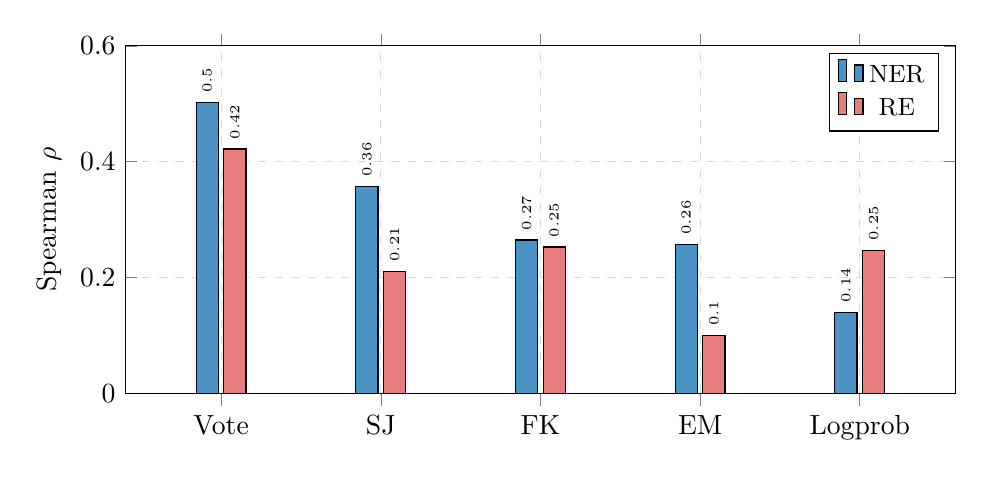
\begin{tikzpicture}
\begin{axis}[
    width=\linewidth,
    height=6cm,
    ybar=2pt,
    bar width=8pt,
    ylabel={Spearman $\rho$},
    symbolic x coords={Vote,SJ,FK,EM,Logprob},
    xtick=data,
    ymin=0, ymax=0.6,
    legend style={at={(0.98,0.98)},anchor=north east,font=\small},
    enlarge x limits=0.15,
    nodes near coords,
    every node near coord/.append style={font=\tiny,rotate=90,anchor=west},
    grid=major,
    grid style={dashed,gray!30},
]
\addplot[fill=structblue!80] coordinates {(Vote,0.502) (SJ,0.357) (FK,0.265) (EM,0.257) (Logprob,0.140)};
\addplot[fill=logprobred!60] coordinates {(Vote,0.422) (SJ,0.211) (FK,0.253) (EM,0.100) (Logprob,0.247)};
\legend{NER,RE}
\end{axis}
\end{tikzpicture}
\caption{Spearman $\rho$ between confidence signals and instance-level $F_1$ on SciERC (Qwen3-8B, $N{=}8$). Structural signals (Vote, SJ) dominate on NER; on RE, logprob becomes competitive due to compound error degradation of consistency signals.}
\label{fig:rho-comparison}
\end{figure}

% ---- 5.2 Generalization ----
\subsection{Cross-Model and Cross-Dataset Generalization}
\label{sec:results-generalization}

\begin{table}[t]
\centering
\caption{$2{\times}2$ cross-model $\times$ cross-dataset quality estimation (Spearman $\rho$, full set, $N{=}8$). Structural signals outperform logprob in all four configurations. Cross-model $|\Delta\rho| \le 0.006$ on the same dataset.}
\label{tab:2x2-rho}
\small
\begin{tabular}{l ccccc r}
\toprule
Configuration & \textsc{sj} & \textsc{vote} & \textsc{fk} & \textsc{em} & \textsc{logprob} & $n$ \\
\midrule
Qwen $\times$ SciERC   & 0.357 & \textbf{0.502} & 0.265 & 0.257 & 0.140 & 529 \\
Qwen $\times$ CoNLL    & 0.436 & 0.424 & 0.400 & \textbf{0.451} & 0.316 & 2756 \\
LLaMA $\times$ SciERC  & 0.363 & --- & 0.327 & --- & 0.183 & 529 \\
LLaMA $\times$ CoNLL   & \underline{0.431} & 0.426 & 0.428 & 0.431 & 0.307 & 2756 \\
\bottomrule
\end{tabular}
\end{table}

\begin{table}[t]
\centering
\caption{AUROC across the $2{\times}2$ matrix ($N{=}8$). Structural signals lead in 3 of 4 configurations; logprob is competitive only on CoNLL (high-baseline regime with well-calibrated models).}
\label{tab:2x2-auroc}
\small
\begin{tabular}{l ccc l}
\toprule
Configuration & \textsc{sj} & \textsc{vote} & \textsc{logprob} & Best signal \\
\midrule
Qwen $\times$ SciERC  & 0.666 & \textbf{0.728} & 0.559 & Vote 0.728 \\
Qwen $\times$ CoNLL   & \textbf{0.801} & 0.789 & 0.753 & SJ 0.801 \\
LLaMA $\times$ SciERC & 0.702 & \textbf{0.718} & 0.558 & Vote 0.718 \\
LLaMA $\times$ CoNLL  & 0.704 & 0.709 & \textbf{0.761} & Logprob 0.761 \\
\bottomrule
\end{tabular}
\end{table}

To assess generalization, we evaluate all signals across a $2{\times}2$ matrix of models (Qwen3-8B, LLaMA-3.1-8B) and datasets (SciERC, CoNLL-2003).

\paragraph{Spearman $\rho$ (\cref{tab:2x2-rho}).}
Structural signals outperform logprob in all four configurations (structural $>$ logprob rate = 100\%).
Cross-model consistency is remarkably high: on CoNLL, Qwen SJ $\rho{=}0.436$ vs.\ LLaMA SJ $\rho{=}0.431$ ($\Delta{=}0.005$); on SciERC, Qwen SJ $\rho{=}0.357$ vs.\ LLaMA $\rho{=}0.363$ ($\Delta{=}{-}0.006$).
Both models exhibit the same dataset effect (CoNLL $>$ SciERC), confirming that consistency signal strength is a task property, not a model artifact.

\paragraph{AUROC (\cref{tab:2x2-auroc}).}
Structural signals achieve the highest AUROC in 3 of 4 configurations.
The exception is LLaMA $\times$ CoNLL, where logprob AUROC (0.761) exceeds structural signals (SJ 0.704, Vote 0.709).
This occurs in the high-baseline regime (greedy $F_1{=}0.927$): when model performance is near-perfect, log-probability calibration is tight and threshold-based classification (AUROC) favors the well-calibrated signal.
However, logprob's \emph{ranking} ability ($\rho{=}0.307$) remains substantially below structural signals ($\rho{=}0.431$).
This AUROC--$\rho$ divergence illustrates why multiple evaluation metrics are necessary: AUROC measures threshold classification while $\rho$ measures rank discrimination.

\begin{figure}[t]
\centering
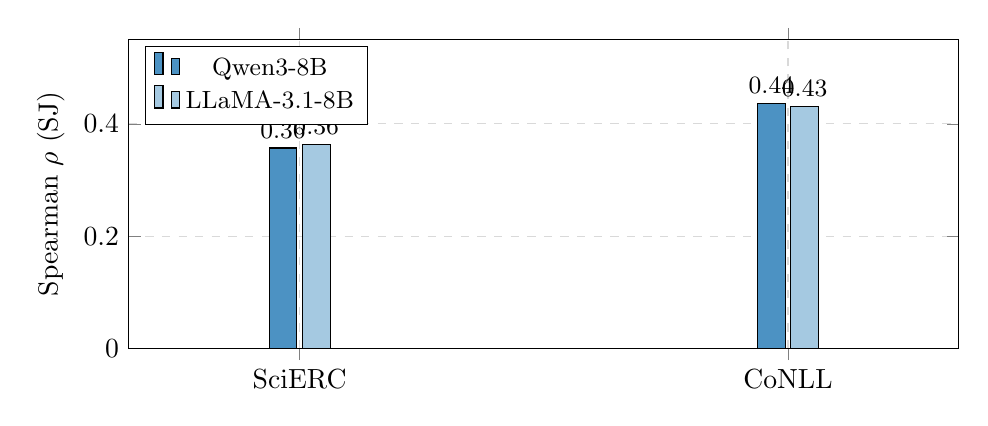
\begin{tikzpicture}
\begin{axis}[
    width=\linewidth,
    height=5.5cm,
    ybar=2pt,
    bar width=10pt,
    ylabel={Spearman $\rho$ (SJ)},
    symbolic x coords={SciERC,CoNLL},
    xtick=data,
    ymin=0, ymax=0.55,
    legend style={at={(0.02,0.98)},anchor=north west,font=\small},
    enlarge x limits=0.35,
    nodes near coords,
    every node near coord/.append style={font=\small},
    grid=major,
    grid style={dashed,gray!30},
]
\addplot[fill=structblue!80] coordinates {(SciERC,0.357) (CoNLL,0.436)};
\addplot[fill=structblue!40] coordinates {(SciERC,0.363) (CoNLL,0.431)};
\legend{Qwen3-8B, LLaMA-3.1-8B}
\end{axis}
\end{tikzpicture}
\caption{Cross-model consistency of Soft Jaccard $\rho$ across datasets. The two architecturally distinct models produce near-identical quality estimation performance ($|\Delta\rho| \le 0.006$), demonstrating that structural consistency is a model-agnostic property.}
\label{fig:cross-model}
\end{figure}

\paragraph{Seed robustness.}
On LLaMA $\times$ CoNLL with $N{=}16$ and three seeds (42, 123, 456), SJ $\rho$ is $0.463 \pm 0.008$, voting $\rho$ is $0.458 \pm 0.003$, and logprob $\rho$ is $0.310 \pm 0.005$ (\cref{tab:robustness}).
The structural--logprob gap is stable across all seeds (structural beats logprob rate = 100\%).
The $N{=}8 \to N{=}16$ improvement is modest for SJ ($+0.033$), suggesting near-saturation on CoNLL NER.

\begin{table}[t]
\centering
\caption{Three-seed robustness (LLaMA $\times$ CoNLL, $N{=}16$). All structural signals consistently outperform logprob with low variance.}
\label{tab:robustness}
\small
\begin{tabular}{l cccc}
\toprule
Metric & Seed 42 & Seed 123 & Seed 456 & Mean $\pm$ Std \\
\midrule
SJ $\rho$       & 0.464 & 0.470 & 0.455 & $0.463 \pm 0.008$ \\
FK $\rho$       & 0.457 & 0.459 & 0.448 & $0.455 \pm 0.006$ \\
Logprob $\rho$  & 0.306 & 0.316 & 0.308 & $0.310 \pm 0.005$ \\
Vote $\rho$     & 0.455 & 0.461 & 0.457 & $0.458 \pm 0.003$ \\
SJ AUROC        & 0.739 & 0.740 & 0.729 & $0.736 \pm 0.006$ \\
\bottomrule
\end{tabular}
\end{table}

% ---- 5.3 Correlation-Selection Gap ----
\subsection{The Correlation--Selection Gap}
\label{sec:results-gap}

\begin{table}[t]
\centering
\caption{Best-of-$N$ selection on SciERC ($N{=}8$, $T{=}1.0$). Despite strong quality estimation, no signal beats greedy on NER. On RE, only logprob surpasses greedy (+2.4pp), as the sole per-sample signal.}
\label{tab:selection}
\small
\begin{tabular}{l cc}
\toprule
Signal & NER $F_1$ & RE $F_1$ \\
\midrule
Oracle         & 0.769 & 0.561 \\
\midrule
Greedy ($T{=}0$) & \textbf{0.609} & 0.374 \\
Logprob        & 0.609          & \textbf{0.397} \\
Ensemble       & 0.604          & --- \\
SJ             & 0.604          & 0.368 \\
Vote           & 0.596          & 0.338 \\
Random         & 0.580          & 0.338 \\
\bottomrule
\end{tabular}
\end{table}

\begin{figure}[t]
\centering
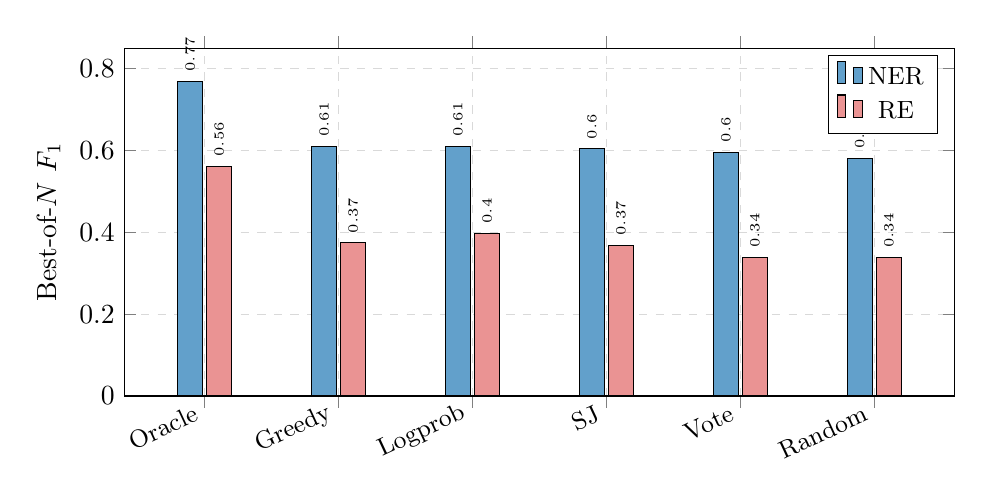
\begin{tikzpicture}
\begin{axis}[
    width=\linewidth,
    height=6cm,
    ybar=1.5pt,
    bar width=9pt,
    ylabel={Best-of-$N$ $F_1$},
    symbolic x coords={Oracle,Greedy,Logprob,SJ,Vote,Random},
    xtick=data,
    x tick label style={rotate=25, anchor=east, font=\small},
    ymin=0.0, ymax=0.85,
    legend style={at={(0.98,0.98)},anchor=north east,font=\small},
    enlarge x limits=0.12,
    nodes near coords,
    every node near coord/.append style={font=\tiny,rotate=90,anchor=west},
    grid=major,
    grid style={dashed,gray!30},
]
\addplot[fill=structblue!70] coordinates {(Oracle,0.769) (Greedy,0.609) (Logprob,0.609) (SJ,0.604) (Vote,0.596) (Random,0.580)};
\addplot[fill=logprobred!50] coordinates {(Oracle,0.561) (Greedy,0.374) (Logprob,0.397) (SJ,0.368) (Vote,0.338) (Random,0.338)};
\legend{NER,RE}
\end{axis}
\end{tikzpicture}
\caption{Best-of-$N$ selection results on SciERC. On NER (blue), no signal surpasses greedy despite large oracle headroom (+16pp). On RE (red), only logprob exceeds greedy (+2.4pp). The gap between oracle and best achievable signal visualizes the \emph{correlation--selection gap}.}
\label{fig:selection}
\end{figure}

\Cref{tab:selection} and \cref{fig:selection} reveal the central finding of this work.
On NER, despite voting's strong quality estimation ($\rho{=}0.502$, AUROC${=}0.728$), its best-of-$N$ selection ($F_1{=}0.596$) \emph{underperforms} greedy decoding ($F_1{=}0.609$).
All consistency signals fail to beat greedy, while the oracle achieves $0.769$ (+16pp headroom).

This gap arises from a fundamental distinction.
Consistency signals are \emph{instance-level aggregates}: they assign one score per input $x$ by measuring agreement across all $N$ samples.
They predict \emph{which inputs are easy vs.\ hard}---ideal for selective prediction and abstention.
But they cannot rank individual samples $y_i$ against each other, which is required for best-of-$N$ selection.

Log-probability is the only \emph{per-sample} signal: it scores each $y_i$ independently.
On RE, where greedy is suboptimal ($F_1{=}0.374$, oracle $0.561$), logprob enables effective selection ($+2.4$pp over greedy).
On NER, where greedy is near-optimal, even logprob provides no benefit.

\paragraph{Practical implications.}
For selective prediction (deciding whether to trust an output), structural consistency signals are the tool of choice.
For best-of-$N$ selection (choosing the best output), log-probability is the only viable unsupervised signal---and only on tasks where greedy decoding is sufficiently suboptimal.
For NER with fine-tuned models, greedy decoding is near-optimal and multi-sample selection adds no value with current signals.

\paragraph{Ensemble analysis.}
Combining signals via logistic regression yields NER AUROC $0.735$ ($+0.7$pp over voting alone) and RE AUROC $0.719$ ($-0.2$pp, no improvement).
A linear combination of SJ and voting achieves optimal NER $\rho{=}0.489$ at $\alpha{=}0.3$.
FK receives a negative coefficient in the logistic model, indicating that surface agreement is net-negative when structural signals are present.
These results suggest that voting captures nearly all discriminative information; ensemble gains are marginal.

% ---- 5.4 Task-Complexity Boundary ----
\subsection{Task-Complexity Boundary}
\label{sec:results-boundary}

All signals degrade from NER to RE (\cref{tab:qe-scierc}).
SJ drops from $\rho{=}0.357$ (NER) to $0.211$ (RE) on the full set---a $-0.146$ decline.
This degradation reflects compound error propagation in relational tasks: RE requires correctly identifying both head and tail entities \emph{and} the relation type.
Errors in any component disrupt consistency measurement.

Conditional filtering (retaining only instances where $F_1 > 0$) substantially restores signal strength.
On RE, SJ recovers from $0.211$ to $0.368$ ($+0.157$), and voting from $0.422$ to $0.463$ ($+0.041$).
The conditional lift dwarfs temperature tuning effects ($\Delta\rho \le \pm 0.01$ across $T{=}0.7/1.0$).
This indicates that the NER--RE gap is primarily a \emph{capability boundary} effect: consistency signals work well within the model's knowledge range but cannot diagnose systematic knowledge gaps.

\paragraph{Temperature analysis.}
SJ exhibits remarkable temperature robustness ($\Delta\rho{=}\pm 0.01$ between $T{=}0.7$ and $T{=}1.0$), while FK is sensitive ($\Delta\rho{=}\pm 0.06$--$0.09$).
$T{=}1.0$ preserves more oracle headroom (RE: $0.167$ vs.\ $0.131$) and output diversity ($1{-}\text{SJ}$: $0.389$ vs.\ $0.313$).
We recommend $T{=}1.0$ with conditional filtering over temperature optimization.

\paragraph{Sample budget scaling.}
Preliminary results ($n{=}200$ subset) suggest that $N{=}8 \to N{=}16$ substantially improves RE signals (voting $\rho$: $0.340 \to 0.448$, $+0.108$) while NER saturates (voting $\rho$: $0.392 \to 0.401$).
This is consistent with the task-complexity interpretation: compound error propagation increases per-instance variance, requiring more samples to average out.
Full-set confirmation of this scaling pattern is left to future work.


% ============================================================
% 6. DISCUSSION
% ============================================================
\section{Discussion}

\paragraph{When does consistency outperform log-probability?}
Our results show a clear advantage for structural consistency under two conditions: (a)~moderate model performance where log-probability calibration is unreliable, and (b)~complex structured outputs where surface metrics fail.
We expect structural signals to further outperform logprob when: (i)~models are used in-context without fine-tuning (poorer calibration); (ii)~log-probabilities are unavailable (closed-source APIs); (iii)~the model is systematically overconfident.
The OOD experiment (\cref{sec:ood}) provides direct evidence: under domain shift, logprob correlation becomes \emph{negative} ($\rho{=}{-}0.031$) while structural signals retain a positive, albeit weak, signal ($\rho{=}0.078$--$0.093$).

\paragraph{AUROC--$\rho$ divergence.}
On LLaMA $\times$ CoNLL, logprob achieves the highest AUROC (0.761) but the lowest $\rho$ (0.307) among structural signals.
AUROC measures threshold classification (``is this above/below median quality?''), while $\rho$ measures rank discrimination (``which is better than which?'').
In the near-perfect regime (greedy $F_1{=}0.927$), logprob calibration is tight and thresholding works well.
But for \emph{ranking} instances---the prerequisite for both selective prediction and sample selection---structural signals remain superior.
This underscores the importance of evaluating quality estimation with multiple metrics.

\paragraph{Limitations.}
Our study has several limitations.
\emph{Model scale}: We evaluate only 8B-parameter models; larger models (70B+) may exhibit different calibration properties that alter the structural--logprob balance.
\emph{Dataset coverage}: We evaluate NER on two datasets and RE on one (SciERC). Informal text domains (social media, conversational) are not covered; the OOD experiment (\cref{sec:ood}) suggests substantial degradation in mismatched domains.
\emph{Selection gap}: We identify the correlation--selection gap but do not resolve it. Developing consistency-based per-sample selection signals (e.g., leave-one-out consistency scoring) is an important direction.
\emph{Supervised baselines}: We compare only unsupervised signals. Trained reward models or verifiers~\cite{cobbe2021training,lightman2023lets} likely outperform all unsupervised approaches; our contribution is the systematic comparison within the unsupervised regime.

% ============================================================
% 7. CONCLUSION
% ============================================================
\section{Conclusion}

We conducted a systematic comparison of five confidence signals for LLM-based information extraction across two models and two datasets.
Structural consistency signals---entity voting confidence and Soft Jaccard---provide the strongest quality estimation, achieving AUROC 0.73 and $\rho{=}0.50$ on NER, substantially outperforming log-probability (AUROC 0.56, $\rho{=}0.14$).
This advantage holds across a $2{\times}2$ model--dataset matrix with cross-model variation $|\Delta\rho|{\le}0.006$ and three-seed standard deviation $\sigma_\rho{\le}0.008$.

We identified a correlation--selection gap: despite strong instance-level quality prediction, no unsupervised consistency signal beats greedy decoding for NER best-of-$N$ selection.
Only per-sample log-probability enables selection on RE, where greedy decoding is suboptimal.
This distinction between quality estimation (``which inputs are reliable?'') and sample selection (``which output is best?'') has direct implications for system design: use structural consistency for selective prediction/abstention, and log-probability for sample selection when applicable.

All signals degrade on relational tasks due to compound error propagation, but conditional filtering restores discriminative power.
These findings provide actionable guidance for deploying multi-sample IE systems and highlight the need for per-sample structural consistency metrics to close the selection gap.

% ============================================================
% APPENDIX
% ============================================================
\appendix
\section{Out-of-Domain Evaluation}
\label{sec:ood}

To assess robustness under domain shift, we evaluate the SciERC-fine-tuned Qwen3-8B on the WNUT-2017 social media NER test set ($n{=}1{,}287$; $n{=}689$ valid after filtering; $n{=}378$ conditional).
Entity type schemas are disjoint (SciERC: Task/Method/Material/Metric; WNUT: person/location/corporation/creative-work), creating a challenging zero-shot transfer scenario.

Greedy $F_1$ drops from 0.66 (SciERC in-domain) to 0.143, with 61.4\% of instances producing $F_1{=}0$.
All quality estimation signals degrade substantially (\cref{tab:ood}).
On the full set, all correlations are near zero ($\rho \le 0.093$), with logprob turning negative ($\rho{=}{-}0.031$).

Two observations are noteworthy.
First, the \emph{relative ordering} of signals is preserved: voting $>$ SJ $>$ FK $>$ EM $>$ logprob, identical to the in-domain ranking.
This suggests that structural consistency is not a dataset-specific artifact.
Second, logprob's negative correlation reflects calibration failure under domain shift: the model assigns confidently high probabilities to incorrect entity types.
Structural signals, which measure inter-sample agreement rather than model confidence, are immune to this miscalibration---they are weak but positive.

On the conditional set (excluding $F_1{=}0$ instances), signals recover partially (SJ $\rho{=}0.198$, voting $\rho{=}0.224$), following the same pattern as in-domain conditional analysis.

\begin{table}[t]
\centering
\caption{OOD quality estimation: SciERC $\to$ WNUT-2017 (Qwen3-8B, $N{=}8$). All signals degrade substantially, but structural signals retain positive correlation while logprob turns negative.}
\label{tab:ood}
\small
\begin{tabular}{l cccc}
\toprule
& \multicolumn{2}{c}{Full ($n{=}689$)} & \multicolumn{2}{c}{Conditional ($n{=}378$)} \\
\cmidrule(lr){2-3} \cmidrule(lr){4-5}
Signal & $\rho$ & AUROC & $\rho$ & AUROC \\
\midrule
\textsc{vote}    & 0.093  & 0.574 & 0.224 & 0.631 \\
\textsc{sj}      & 0.078  & 0.562 & 0.198 & 0.618 \\
\textsc{fk}      & 0.064  & 0.548 & 0.152 & 0.594 \\
\textsc{em}      & 0.051  & 0.539 & 0.141 & 0.587 \\
\textsc{logprob} & $-$0.031 & 0.487 & 0.117 & 0.573 \\
\bottomrule
\end{tabular}
\end{table}

% ============================================================
% REFERENCES
% ============================================================
\begin{thebibliography}{35}
\bibitem[Wang et al.(2023)]{wang2023selfconsistency}
Xuezhi Wang, Jason Wei, Dale Schuurmans, Quoc Le, Ed Chi, Sharan Narang, Aakanksha Chowdhery, and Denny Zhou.
Self-consistency improves chain of thought reasoning in language models.
In \emph{ICLR}, 2023.

\bibitem[Snell et al.(2024)]{snell2024scaling}
Charlie Snell, Jaehoon Lee, Kelvin Xu, and Aviral Kumar.
Scaling LLM test-time compute optimally can be more effective than scaling model parameters.
\emph{arXiv:2408.03314}, 2024.

\bibitem[Brown et al.(2024)]{brown2024tts}
Bradley Brown, Jordan Juravsky, Ryan Ehrlich, Ronald Clark, Quoc V. Le, Christopher R\'{e}, and Azalia Mirhoseini.
Large language monkeys: Scaling inference compute with repeated sampling.
\emph{arXiv:2407.21787}, 2024.

\bibitem[Chen et al.(2024)]{chen2024usc}
Xinyun Chen, Renat Aksitov, Uri Alon, Jie Ren, Kefan Xiao, Pengcheng Yin, Sushant Prakash, Charles Sutton, Xuezhi Wang, and Denny Zhou.
Universal self-consistency for large language model generation.
\emph{arXiv:2311.17311}, 2024.

\bibitem[Kuhn et al.(2023)]{kuhn2023semantic}
Lorenz Kuhn, Yarin Gal, and Sebastian Farquhar.
Semantic uncertainty: Linguistic invariances for uncertainty estimation in natural language generation.
In \emph{ICLR}, 2023.

\bibitem[Kadavath et al.(2022)]{kadavath2022language}
Saurav Kadavath, Tom Conerly, Amanda Askell, et al.
Language models (mostly) know what they know.
\emph{arXiv:2207.05221}, 2022.

\bibitem[Guo et al.(2017)]{guo2017calibration}
Chuan Guo, Geoff Pleiss, Yu Sun, and Kilian Q. Weinberger.
On calibration of modern neural networks.
In \emph{ICML}, 2017.

\bibitem[Desai and Durrett(2020)]{desai2020calibration}
Shrey Desai and Greg Durrett.
Calibration of pre-trained transformers.
In \emph{EMNLP}, 2020.

\bibitem[Fisch et al.(2021)]{fisch2021conformal}
Adam Fisch, Tal Schuster, Tom{\'a}s Jaakkola, and Regina Barzilay.
Few-shot conformal prediction with auxiliary tasks.
In \emph{ICML}, 2021.

\bibitem[Angelopoulos et al.(2021)]{angelopoulos2021gentle}
Anastasios N. Angelopoulos and Stephen Bates.
A gentle introduction to conformal prediction and distribution-free uncertainty quantification.
\emph{arXiv:2107.07511}, 2021.

\bibitem[Xiao and Wang(2019)]{xiao2019quantifying}
Yijun Xiao and William Yang Wang.
Quantifying uncertainties in natural language processing tasks.
In \emph{AAAI}, 2019.

\bibitem[Shelmanov et al.(2021)]{shelmanov2021certain}
Artem Shelmanov, Evgenii Tsymbalov, Dmitri Puzyrev, Kirill Fedyanin, Alexander Panchenko, and Maxim Panov.
How certain is your transformer?
In \emph{EACL}, 2021.

\bibitem[Lakshminarayanan et al.(2017)]{lakshminarayanan2017simple}
Balaji Lakshminarayanan, Alexander Pritzel, and Charles Blundell.
Simple and scalable predictive uncertainty estimation using deep ensembles.
In \emph{NeurIPS}, 2017.

\bibitem[Gal and Ghahramani(2016)]{gal2016dropout}
Yarin Gal and Zoubin Ghahramani.
Dropout as a {B}ayesian approximation: Representing model uncertainty in deep learning.
In \emph{ICML}, 2016.

\bibitem[Cobbe et al.(2021)]{cobbe2021training}
Karl Cobbe, Vineet Kosaraju, Mohammad Bavarian, Mark Chen, Heewoo Jun, Lukasz Kaiser, Matthias Plappert, Jerry Tworek, Jacob Hilton, Reiichiro Nakano, Christopher Hesse, and John Schulman.
Training verifiers to solve math word problems.
\emph{arXiv:2110.14168}, 2021.

\bibitem[Lightman et al.(2023)]{lightman2023lets}
Hunter Lightman, Vineet Kosaraju, Yura Burda, Harri Edwards, Bowen Baker, Teddy Lee, Jan Leike, and John Schulman.
Let's verify step by step.
In \emph{ICLR}, 2024.

\bibitem[Kuleshov and Liang(2015)]{kuleshov2015structured}
Volodymyr Kuleshov and Percy Liang.
Calibrated structured prediction.
In \emph{NeurIPS}, 2015.

\bibitem[Jagannatha and Yu(2022)]{jagannatha2022calibration}
Abhyuday Jagannatha and Hong Yu.
Calibrating structured output predictors for natural language processing.
In \emph{ACL}, 2022.

\bibitem[Culotta and McCallum(2004)]{culotta2004confidence}
Aron Culotta and Andrew McCallum.
Confidence estimation for information extraction.
In \emph{HLT-NAACL}, 2004.

\bibitem[Manakul et al.(2023)]{manakul2023selfcheckgpt}
Potsawee Manakul, Adian Liusie, and Mark J.F. Gales.
{S}elf{C}heck{GPT}: Zero-resource black-box hallucination detection for generative large language models.
In \emph{EMNLP}, 2023.

\bibitem[Geifman and El-Yaniv(2017)]{geifman2017selective}
Yonatan Geifman and Ran El-Yaniv.
Selective classification for deep neural networks.
In \emph{NeurIPS}, 2017.

\bibitem[N\'{e}dellec and Xia(2026)]{nedellec2026consistency}
Claire N\'{e}dellec and Haoling Xia.
Consistency--accuracy correlation in hard-prompted {LLM}s for entity and relation extraction.
\emph{Genomics Informatics}, 2026.

\bibitem[CISC(2025)]{cisc2025}
Confidence-weighted self-consistency for reasoning.
In \emph{ACL Findings}, 2025.

\bibitem[Self-Certainty(2026)]{selfcertainty2026}
Self-certainty best-of-{N}: Reward-free selection via {KL}-divergence.
In \emph{ICLR}, 2026.

\bibitem[ReASC(2026)]{reasc2026}
Reliability-aware adaptive self-consistency.
\emph{arXiv:2601.02970}, 2026.

\bibitem[Atomic SC(2024)]{atomic2024}
Atomic self-consistency for better long form generations.
In \emph{EMNLP}, 2024.

\bibitem[UQ Survey(2025)]{uqsurvey2025}
Uncertainty quantification for large language models: A survey.
In \emph{ACL Findings}, 2025.

\bibitem[UQ+Calibration Survey(2025)]{uqcalibsurvey2025}
Uncertainty quantification and calibration for large language models.
\emph{arXiv:2503.15850}, 2025.

\bibitem[Semantic Probes(2024)]{semanticprobes2024}
Semantic entropy probes: Robust and cheap hallucination detection in {LLM}s.
2024.

\bibitem[Latent SC(2025)]{latentsc2025}
Latent self-consistency: Uncertainty estimation in embedding space.
\emph{arXiv:2508.18395}, 2025.

\bibitem[Ranked Voting(2025)]{rankedvoting2025}
Ranked voting self-consistency.
\emph{arXiv:2505.10772}, 2025.

\bibitem[CoCoA(2025)]{cocoa2025}
Misha Vashurin, Mariya Lysyuk, Artem Vazhentsev, Alexander Panchenko, and Maxim Panov.
{CoCoA}: Combining confidence and consistency for uncertainty quantification.
In \emph{NeurIPS}, 2025.

\bibitem[Vashurin et al.(2025)]{vashurin2025eval}
Misha Vashurin et al.
Systematic evaluation of uncertainty quantification methods for large language models.
\emph{arXiv:2510.20460}, 2025.

\bibitem[Know Your Limits(2025)]{knowyourlimits2025}
Know your limits: A survey on abstention in large language models.
In \emph{TACL}, 2025.

\bibitem[Conf. Estimation Survey(2024)]{confestsurvey2024}
Confidence estimation survey for large language models.
\emph{arXiv:2311.08298}, 2024.

\bibitem[Luan et al.(2018)]{luan2018multi}
Yi Luan, Luheng He, Mari Ostendorf, and Hannaneh Hajishirzi.
Multi-task identification of entities, relations, and coreference for scientific knowledge graph construction.
In \emph{EMNLP}, 2018.

\bibitem[Tjong Kim Sang and De Meulder(2003)]{conll2003}
Erik F. Tjong Kim Sang and Fien De Meulder.
Introduction to the {CoNLL}-2003 shared task: Language-independent named entity recognition.
In \emph{CoNLL}, 2003.

\bibitem[Derczynski et al.(2017)]{derczynski2017wnut}
Leon Derczynski, Eric Nichols, Marieke van Erp, and Nut Limsopatham.
Results of the {WNUT}2017 shared task on novel and emerging entity recognition.
In \emph{W-NUT Workshop}, 2017.

\bibitem[Qwen Team(2025)]{qwen2025}
Qwen Team.
Qwen3 technical report.
2025.

\bibitem[LLaMA Team(2024)]{llama2024}
Meta AI.
The {L}lama 3 herd of models.
\emph{arXiv:2407.21783}, 2024.

\end{thebibliography}

\end{document}
